\appendix

\section{Dataset Specifications}
We list the specifications of train/validation/test split of the two datasets (six categories) in Table~\ref{Amazon-Spec}~and Table~\ref{Lazada-Spec}.
The numbers ``$X/Y$'' represent that the split contains $X$ product descriptions and $Y$ reviews.
Amazon-MRHP is an pure English dataset, while Lazada-MRHP is written in Indonesian so that we do not conduct BERT related experiments on it.
\begin{table}[ht]
    \centering
    \small
    \resizebox{\linewidth}{!}{
    \begin{tabularx}{0.5\textwidth}{lccc}
        \toprule
        \multicolumn{4}{c}{\textbf{Amazon-MRHP (Products/Reviews)}} \\
        [0.5ex]
        Cat. & Cloth. \& Jew. & Elec. & Home \& Kitch.\\
        \midrule
        Train & 12,074/277,308  & 10,564/240,505 & 14,570/369,518 \\
        Dev &  3,019/122,148 & 2,641/84,402 & 3,616/92,707 \\
        Test & 3,966/87,492 & 3,327/79,750  &  4,529/111,593 \\
        \bottomrule
    \end{tabularx}
    }
    \caption{Statistics of the Amazon-MRHP dataset.}
    \label{Amazon-Spec}
\end{table}

\begin{table}[ht]
    \centering
    \small
    \resizebox{\linewidth}{!}{
    \begin{tabularx}{0.5\textwidth}{lccc}
        \toprule
        \multicolumn{4}{c}{\textbf{Lazada-MRHP (Products/Reviews)}} \\
        [0.5ex]
        Cat. & Cloth. \& Jew. & Elec. & Home \& Kitch.\\
        \midrule
        Train & 6,596/10,4093 & 3,848/41,828 &  2,939/36,991 \\
        Dev & 1,649/26,139 & 963/10,565 & 736/9,611 \\
        Test & 2,062/32,274 & 1,204/12,661 & 920/12,551 \\
        \bottomrule
    \end{tabularx}
    }
    \caption{Statistics of the Lazada-MRHP dataset.}
    \label{Lazada-Spec}
\end{table}

\section{Training Details}
\subsection{Initialization of Embeddings}
To stay consistent with previous works, we embed the text input of Amazon-MRHP with GloVe-300d~\cite{pennington2014glove} and Lazada-MRHP with  Fasttext~\cite{joulin2016fasttext}, respectively.
In BERT-related experiments we employ the Huggingface toolkit for pretrained models\footnote{https://huggingface.co/docs/transformers/index}.

\subsection{Hyperparameter Search space}
The optimal hyperparameter settings are listed in Table \ref{Amazon hyperparameters}, \ref{lazada hyperparameters} and \ref{Amazon Bert hyperparameters}.
The search space of these hyperparameters are: learning rate in $\{1e^{-4}, 5e^{-4}\}$, text embedding dropout fixed at $\{0.2\}$, shared space hidden dimension in $\{128, 256\}$.

\begin{table}[ht!]
    \centering
    \resizebox{\linewidth}{!}{\begin{tabular}{lccc}
    \toprule
    \multicolumn{4}{c}{\textbf{Amazon-MRHP Glove Hyperparameters}} \\
         & Cloth. \& Jew. &  Elec. & Home \& Kitch. \\
         \midrule
         learning rate  & $1e^{-4}$  & $5e^{-4}$ & $5e^{-4}$ \\
         text embedding dim & 300 & 300 & 300 \\
         text embedding dropout & 0.2 & 0.2 & 0.2 \\
         image embedding dim & 256 & 256 & 256 \\
         text embedding dim & 128 & 128 & 128 \\
         shared space hidden & 128 & 128 & 128 \\
         $r$ & 4 & 4 & 4 \\
         K & 96 & 128 & 64 \\
         batch size & 32 & 32 & 32 \\
         \bottomrule
    \end{tabular}
    }
    \caption{Hyperparameters for Amazon-MRHP using glove-300d embeddings.}
    \label{Amazon hyperparameters}
\end{table}

\begin{table}[ht!]
    \centering
    \resizebox{\linewidth}{!}{\begin{tabular}{lccc}
    \toprule
    \multicolumn{4}{c}{\textbf{Lazada-MRHP fastText Hyperparameters}} \\
         & Cloth. \& Jew. &  Elec. & Home \& Kitch. \\
         \midrule
         learning rate  & $1e^{-4}$  & $5e^{-4}$ & $1e^{-4}$ \\
         text embedding dropout & 0.2 & 0.2 & 0.2 \\
         image embedding dim & 256 & 256 & 256 \\
         text embedding dim & 128 & 128 & 128 \\
         shared space hidden & 128 & 128 & 128 \\
          $r$ & 4 & 4 & 4 \\
          $K$ & 96 & 96 & 128 \\
         batch size & 32 & 32 & 32 \\
         \bottomrule
    \end{tabular}
    }
    \caption{Hyperparameters for Lazada-MRHP using fasttext embeddings.}
    \label{lazada hyperparameters}
\end{table}

\begin{table}[ht!]
    \centering
    \resizebox{\linewidth}{!}{\begin{tabular}{lccc}
    \toprule
    \multicolumn{4}{c}{\textbf{Amazon-MRHP BERT Hyperparameters}} \\
         & Cloth. \& Jew. &  Elec. & Home \& Kitch. \\
         \midrule
         learning rate  & $1e^{-5}$  & $1e^{-5}$ & $1e^{-5}$ \\
         bert learning rate &  $1e^{-5}$  & $1e^{-5}$ & $1e^{-5}$ \\
         text embedding dropout & 0.2 & 0.2 & 0.2 \\
         image embedding dim & 512 & 512 & 512 \\
         text embedding dim & 256 & 256 & 256 \\
         shared space hidden & 256 & 256 & 256 \\
          $r$ & 4 & 4 & 4 \\
          $K$ & 128 & 128 & 128 \\
         batch size & 16 & 16 & 8 \\
         \bottomrule
    \end{tabular}
    }
    \caption{Hyperparameters for all categories using BERT as encoder}
    \label{Amazon Bert hyperparameters}
\end{table}



% \subsection{Hardware Settings}
% We train and test both datasets on a single NVIDIA RTX A6000 GPU.
% The gradients are calculated and backpropagated for each batch in a single forward pass, without batch division and gradient accumulation.
\label{sec:appendix}

\subsection{Sampling of Production Description-Review Pairs in Training}
We mentioned in~\cref{sec:Training} that the training pairs are sampled from the training set.
Now we describe how do we sample these training pairs.
% \todo{Complete this section}
First, we sample $B$ products from the training set where $B$ is the batch size.
Next, for each product, we randomly sample one of its positive review (rating is greater than 2 and $N_r^{-}$ negative reviews (rating is less than or equal to 2 from the corresponding review set.
The dataset has been filtered during manufacture time so that there is always at least one positive/negative review under each product.
To put it in a nutshell, a sampled batch contains $B$ product descriptions, $B$ positive reviews and $N_r^{-}B$ negative reviews.

\section{The Differentiability of top-K Operation in PyTorch}
Given a vector $S = \{s_1, s_2, ..., s_L\} \in \mathbb{R}^L$ where $L$ is the length of that vector, when passing through the top-K operation, most fundamentally its largest $K$ values are selected and sorted in descending order to form a new vector $T = \{t_1, t_2, ..., t_K\} \in \mathbb{R}^K$. 
Suppose the indices of $T$'s elements in $S$ are $I= \{i_1, i_2, ..., i_K\} \subset \{1, 2, ..., L\}$, then the process equals to that concurrently there is a mask $M \in \{0,1\}^L $ automatically created and ``multiplies'' on $S$. 
Each value $m_j$ in $M$ is
\begin{equation*}
    m = 
    \begin{cases}
        1, \quad if \quad j \in I \\
        0, \quad if \quad j \notin I
    \end{cases}
\end{equation*}
With this mask, the forward and backward propagation can proceed as in conventional routines.

\section{Training Speed}
\subsection{Theoretical Analysis}
For simplicity, we consider the case of a pair of modality sequence.
Let $X_1\in \mathbb{R}^{l_1\times d}$, $X_2\in \mathbb{R}^{l_2\times d}$ be a pair of input modality sequences. Here we assume they have been both projected to the same dimension as a common practice that both the fusion--prediction routines and our matching approach exercise.
The multihead attention operation in fusion-based models can be written as:
\begin{equation}
    X_{12} = Att(X_1,X_2)
\end{equation}
Note that attention is a \textit{directional} operation, i.e. $Att(M_1,M_2)\neq Att(M_2,M_1)$. 
Due to this, a fusion-based learning model $\mathcal{M}$ always adopts a pair of conjugate attention. Therefore, for a model of $N$ layers, the total computational complexity $C_f$ is:
\begin{equation}
    C_{f}=(2l_1l_2+l_1^2+l_2^2)Nd
\end{equation}

Now consider matching-based models. 
We only have self-attention for each modality per layer. 
The whole computational complexity consists of the self-attention (att) and multi-scale matching score (mm).
\begin{equation}
    C_{m} = C_{att} + C_{mm}
\end{equation}
Since the number of scales decreases as the aggregation proceeds, we denote the decreasing ratio at layer $i$ for modality $j$ as $k_{i,j}$. Hence, the total computational complexity is:
\begin{equation}
    C_{att}=2\sum_pl_p^2d\left(1+\frac{1}{k_{p,1}^2}+\frac{1}{k_{1,p}^2k_{2,p}^2}+...\right) 
\end{equation}
In our settings, $k_{p,1}$ is large (typically greater than 10), therefore $\frac{1}{k_{p,j}^2} < 0.01$ and can be ignored:
\begin{equation}
    C_{att} = 2(l_1^2+l_2^2)d
\end{equation}
As for the second term, we have:
\begin{equation}
\begin{split}
    C_{mm} &=  l_1\left(\frac{1}{k_{1,1}}+...\right)l_2\left(\frac{1}{k_{2,1}}+...\right)d \\
    &< \frac{l_1l_2d}{k_{1,1}k_{2,1}(1-k_1^{-1})(1-k_2^{-1})} \\
\end{split}
\end{equation}
In the MRHP dataset, $l_1\approx l_2 = l$. 
% Thus $C_f=4Nl^2d$ and $C_m=5l^2d$. 
For the typical value $N=2, k_1=k_2=10$, we have $C_f=8l^2d$ and $C_m < (4+\frac{1}{81})l^2d=4.01l^2d$, or 
\begin{equation}
    \frac{C_m}{C_f}\approx0.5
\end{equation}
which is closed to the measured acceleration in~\ref{fig:speedcomp}. In fact, let $C_m=C_f$ and $N=2$, we have $l_1\approx 2.42 l_2$, which seldom happens in the whole dataset. We observe that the number of hot regions is greater than the text length.
    

\subsection{Numerical Results}
We measure the average training time per batch of MCR, SANCL (the state-of-the-art baseline) and PREMISE, as shown in Figure~\ref{fig:speedcomp}.
The average values are calculated by counting the total time of iterations over 100 batches for 5 random intervals during the whole training process. 

Mathematically, denote the counted time of the $i^{th}$ interval as $t_i$, the speed is calculated as follows
\begin{equation}
    speed = \frac{\sum_{i=1}^5 t_i}{100 \times 5} 
\end{equation}
It can be seen that the training time has been greatly shortened by 42\% and 65\% compared to SANCL (the fastest baseline, athough they have closed number of parameters as shown in~\Cref{tab:model_comp}) and GBDT (the strongest baseline), which approximately matches the conclusion given by mathematical deduction. 

\begin{figure}
    \centering
    \resizebox{\linewidth}{!}{
        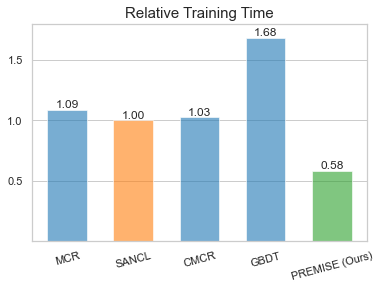
\includegraphics{Contents/img/speed_comp.png}
    }
    \caption{The relative training time of different models. The fastest baseline (SANCL) is highlighted in orange, while our model is highlighted in green. Others are in blue.}
    \label{fig:speedcomp}
\end{figure}

\section{Experiment on Multimodal Retrieval}
We test~\modelname~on multimodal retrieval (bidirectional) task, the results of both image-to-text and text-to-image retrieval on the MSCOCO test set are shown in~\Cref{tab:retrieval}. It can be seen that although our formulation process is completely based on ``learning-from-relation" in MRHP task, the constructed model still has some generalizability to other tasks that our hypothesis stands.

\begin{table*}[t]
    \centering
    \begin{tabular}{c|c|c|c|c}
    \toprule
       \multirow{2}{*}{Model}  & \multicolumn{2}{c|}{Image-to-Text} & \multicolumn{2}{c}{Text-to-Image} \\
    \cline{2-5}
    ~ & PRMP & R@1 & PRMP & R@1 \\ 
    \hline
    VCRN~\cite{li2019visual} & 29.70 & \textbf{53.00} & 29.90 & \textbf{40.50} \\
    PCME~\cite{chun2021probabilistic} & 34.10 & 41.70 & \underline{34.40} & 31.20 \\
    MSRM~\cite{wang2023multilateral} & \textbf{35.62} & \underline{44.32} & \textbf{35.81} & \underline{33.40} \\
    \hline
    \modelname & \underline{34.23} & 42.06 & 33.92 & 31.50 \\
    \bottomrule
    \end{tabular}
    \caption{Results on MSCOCO-5K test set. The highest values in each metric are in bold, while the second-highest are indicated with an underline.}
    \label{tab:retrieval}
\end{table*}

\section{Case Study}
\subsection{How matching scores affect the prediction?}
To further understand the model's functional mechanism, we randomly pick an example from the Amazon--electronics and visualize some matching scores during the test time in Figure~\ref{fig:case_study}.
There are several valuable points to underline.
First, when the model achieves the best performance, its matching scores can reflect the correlation between some semantically matched feature pairs.
For instance, the RoI-RoI matching score of -0.17 is produced by the two RoIs that enclose different objects in their respective images, and thus the correlation between them is very weak, and a near 0 score is obtained, while the two boxes that contain the port hub achieve a relatively high matching score.
Second, text-text matching may act as word matching. 
It is hard to attribute the 0.89 matching score of those two sentences to the high semantic similarity between those two text snippets since their semantic meanings are different, only to share some common words.
These two discoveries reveal that~\modelname~attends to more than semantic matching, and just a certain number of correct matching scores could make up the last features for its accurate prediction, in accord with the conclusion about $K$ values. 

\subsection{Comparison on examples with GBDT}
We further randomly draw two examples which PREMISE gives accurate predictions but GBDT, the state-of-the-art baseline, fails. 
The original review context (including text and attached image) together with the predictions from GBDT and our model towards these two examples are displayed  in~\Cref{tab:elec_product}~to~\Cref{tab:case_study2}. 

We find that~\modelname~ ranks these reviews in correct order (it has the same ranking sequence $1\to 2 \to 3$  and $1 \to 2 \to 3 \to 4$ as the ground truth's in the two examples respectively) even trained and tested with normalized score whose values range from 0 to 1 (different from the annotated scores $s\in [0,4]$). In the given examples, GBDT flips the order of 'B005NGQWL2-9' and 'B005NGQWL2-65' in example 1 and the order of 'B00H4O1L9Y-111' and 'B00H4O1L9Y-122' in example 2.
This could imply that matching-based modeling can make more accurate predictions than fusion-based modeling.

\begin{figure*}
    \centering
    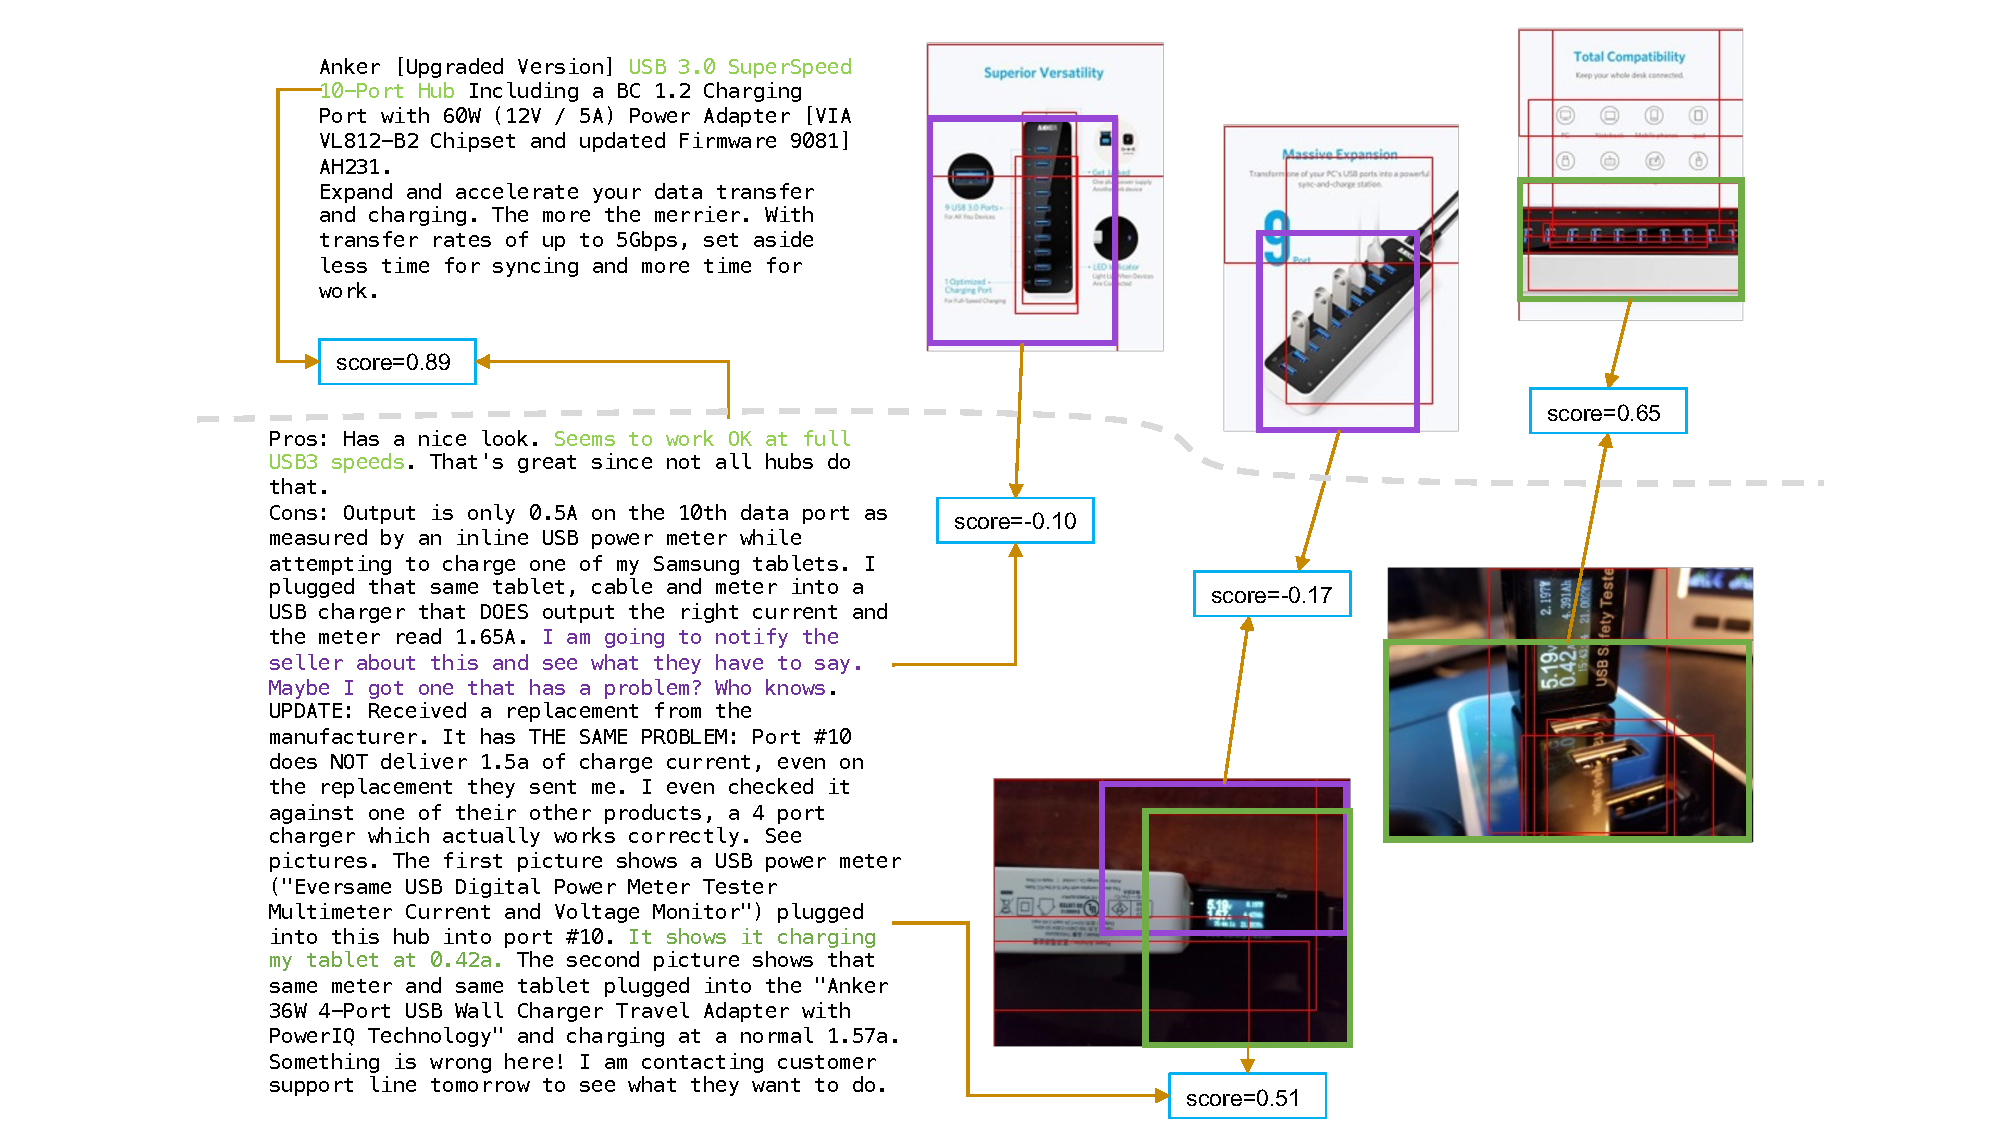
\includegraphics[scale=0.52, trim=2cm 0 0 0]{Contents/img/case_study.pdf}
    \caption{A case study from Amazon-MRHP dataset. 
    The upper and lower part of the figure is the product and review post respectively.
    Green and purple are instance pairs that produce high and low scores that are selected/not selected into the final feature vector. 
    For the matching of n-gram words, we display the largest matching scores between individual words in that scope and the other elements.}
    \label{fig:case_study}
\end{figure*}

\begin{table*}[ht]
    \resizebox{\textwidth}{!}{
        \begin{tabular}{p{0.2\linewidth}|p{0.7\linewidth}}
        \toprule
           Product ID & Introduction \\
         \midrule
            B005NGQWL2 & Expand and accelerate your data transfer and charging. <br><br><b>The more the merrier.</b><br>With transfer rates of up to 5Gbps, set aside less time for syncing and more time for work. With 10 data terminals to choose from, forget about ever having to switch or unplug again.<br><br><b>Fast charging.</b><br>10th-port dual functionality enables fast charges of up to 1.5 amps with BC 1.2 charging-compliant devices, while simultaneously transferring data. Charge via a power adapter for higher 2 amp speeds with all USB-enabled devices when hub is disconnected from an active USB port, or your computer is off or in sleep mode. Dual functions, duly facilitated.<br><br><b>A mainstay for the future.</b><br>Featuring a high-grade chipset and a powerful 60W adapter, this hub ensures a stable power supply while you work. Get steady operation for years to come. Whether at home or in the office, add another can't-do-without fixture to your desk.<br><br><b>BC 1.2 Charging-Compliant Devices:</b><br>Apple: iPhone 5 / 5s, iPad Air, iPad mini / mini 2<br>Samsung: Galaxy S3 / S4, Galaxy Note 1 / 2, Galaxy Mega, Galaxy Mini, Exhilarate, Galaxy Tab 2 10.1<br>Google: Nexus 4 / 5 / 7 / 10<br>Sony: Xperia TX <br>Nokia: Lumia 920, Lumia 1020 <br><br><b>System Requirements</b><br>Windows (32/64 bit) 10 / 8.1 / 8 / 7 / Vista / XP, Mac OS X 10.6-10.9, Linux 2.6.14 or later.<br>Mac OS X Lion 10.7.4 users should upgrade to Mountain Lion 10.8.2 or later to avoid unstable connections.<br><br><b>Compatibility</b><br>2.4GHz wireless devices, MIDI devices and some USB 3.0 devices may not be supported. Try using the host port or a USB 2.0 connection.<br><br><b>Power Usage</b><br>For a stable connection, don't use this hub with high power-consumption devices, such as external hard drives. The hub will sync but not charge tablets and other devices which require a higher power input.

        \subfigure{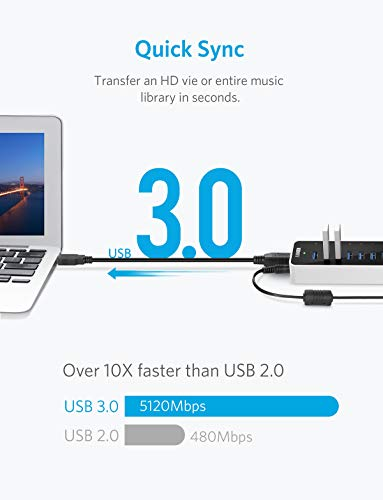
\includegraphics[height=\csfigheight]{Contents/img/case_study/product/pic_6_0.jpg}}
        \subfigure{
\includegraphics[height=\csfigheight]{Contents/img/case_study/product/pic_6_1.jpg}}
        \subfigure{
\includegraphics[height=\csfigheight]{Contents/img/case_study/product/pic_6_2.jpg}}
        \subfigure{
\includegraphics[height=\csfigheight]{Contents/img/case_study/product/pic_6_3.jpg}}
        \subfigure{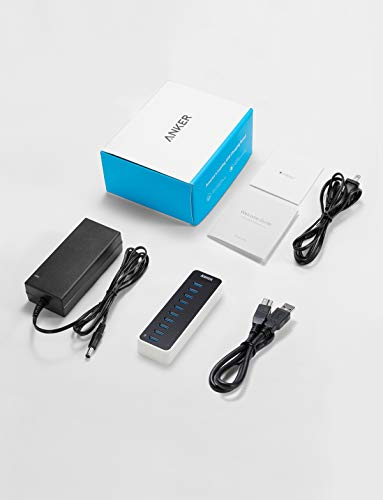
\includegraphics[height=\csfigheight]{Contents/img/case_study/product/pic_6_4.jpg}} 
        \subfigure{
\includegraphics[height=\csfigheight]{Contents/img/case_study/product/pic_6_5.jpg}} 
        \\
        \bottomrule
        \end{tabular}
    }
    \caption{(Example 1 of 2) Product introduction of an example from Amazon Electronics dataset. Some special characters have been removed for better readability.}
    \label{tab:elec_product}
\end{table*}

\begin{table*}[ht!]
    \resizebox{\textwidth}{!}{
        \begin{tabular}{p{0.2\linewidth}|p{0.7\linewidth}|p{0.07\linewidth}|p{0.07\linewidth}|p{0.07\linewidth}}
        \toprule
        Review ID & Content & GT & GBDT & Ours \\
        \midrule
        B005NGQWL2-14 & 
        Pros:
        
        Has a nice look. Seems
        to work OK at full USB3 speeds. That's great since not all hubs do that.
        
        Cons: 

        Output is only 0.5A on the 10th data port as measured by an inline USB power meter while attempting to charge one of my Samsung tablets. I plugged that same tablet, cable and meter into a USB charger that DOES output the right current and the meter read 1.65A. 
        
        I am going to notify the seller about this and see what they have to say. Maybe I got one that has a problem? Who knows. 
        
        UPDATE: Received a replacement from the manufacturer. It has THE SAME PROBLEM: Port \#10 does NOT deliver 1.5A of charge current, even on the replacement they sent me. I even checked it against one of their other products, a 4 port charger which actually works correctly. See pictures. The first picture shows a USB power meter (``Eversame USB Digital Power Meter Tester Multimeter Current and Voltage Monitor") plugged into this hub into port \#10. It shows it charging my tablet at 0.42a. The second picture shows that same meter and same tablet plugged into the "Anker 36W 4-Port USB Wall Charger Travel Adapter with PowerIQ Technology" and charging at a normal 1.57a. Something is wrong here! I am contacting customer support line tomorrow to see what they want to do.
        
        \subfigure{
\includegraphics[height=\csfigheight]{Contents/img/case_study/review3/pic_2_0.jpg}}
        \subfigure{
\includegraphics[height=\csfigheight]{Contents/img/case_study/review3/pic_2_1.jpg}}
        & 3.00 & 0.86 & 0.89 \\
        \midrule
        B005NGQWL2-9 & I rarely write a negative review, in fact almost never. This AnkerDirect 10-Port USB Data hub lasted only about 2 months. Now none of the USB ports work.  For the first couple of weeks all the ports seemed fine. Then one by one they stopped working. Power gets to the unit and the USB ports on my MAC work fine. I've been waiting for a replacement from the company ever since April 20th 2017, after sending their support group my address as requested,  but it had not arrived.
        
        I wish to amend this review by saying that the Anker customer service folks were very helpful in rectifying this situation. After some checks on the original item at their direction, the Anker folks came to the conclusion that I had a defective product and quickly replaced it with a new model. I've had a couple of days to test it out and it appears to be working just fine. I have always felt that a product or service can go bad but it is the company's response to that problem, should it arise, that gains my respect and future business.

        \subfigure{
\includegraphics[height=\csfigheight]{Contents/img/case_study/review2/pic_1_0.jpg}}
        & 2.00 & 0.64 & 0.52 \\
        
        \midrule
        B005NGQWL2-65 & Works very great, powers all of my USB connections, I have a Asus Gaming Laptop which only has 4 USB ports and I needed to have a blue yeti mic, a Logitech Webcam c920,  razer keyboard chroma,  2tb hard drive,  and a Xbox one controller wireless adapter connected to it. 
        
        So far nothing has disconnected or malfunctioned. I would definitely recommend this to my friends and familiy. 
        
        \subfigure{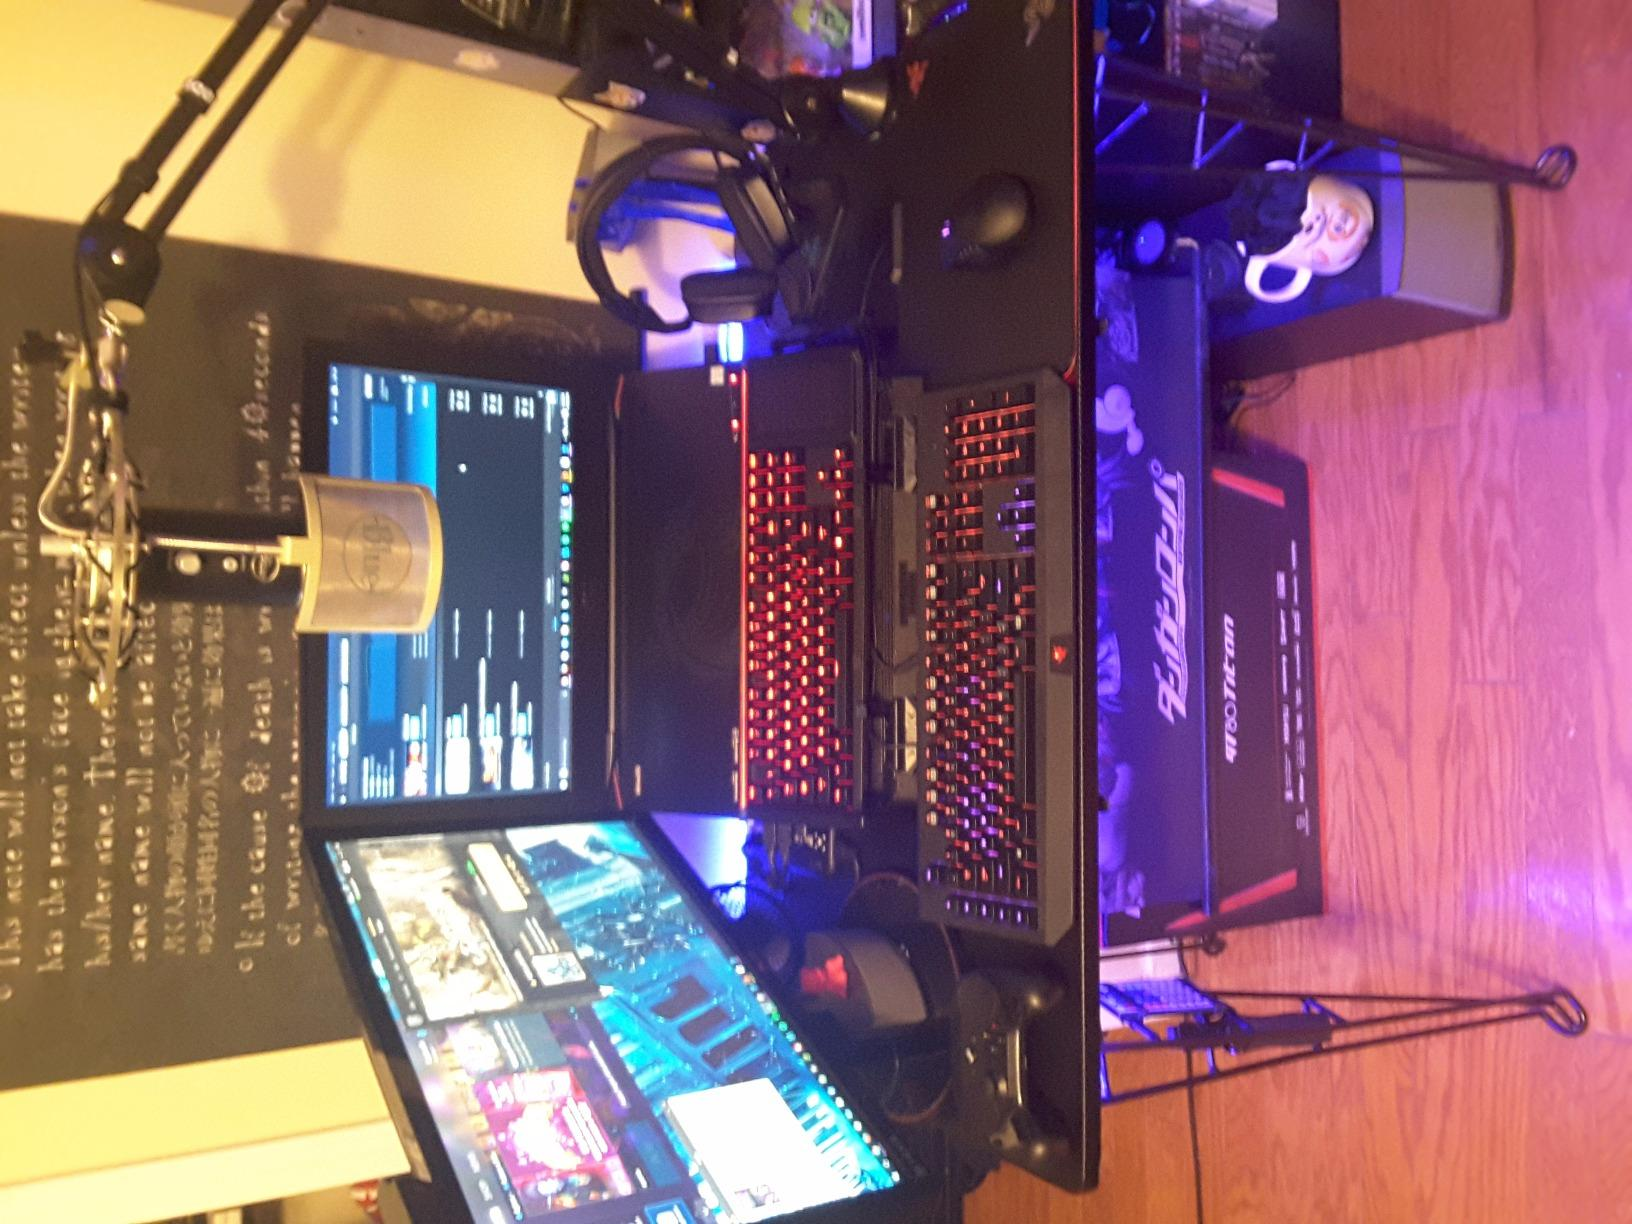
\includegraphics[height=\csfigheight]{Contents/img/case_study/review1/pic_2_0.jpg}}
        \subfigure{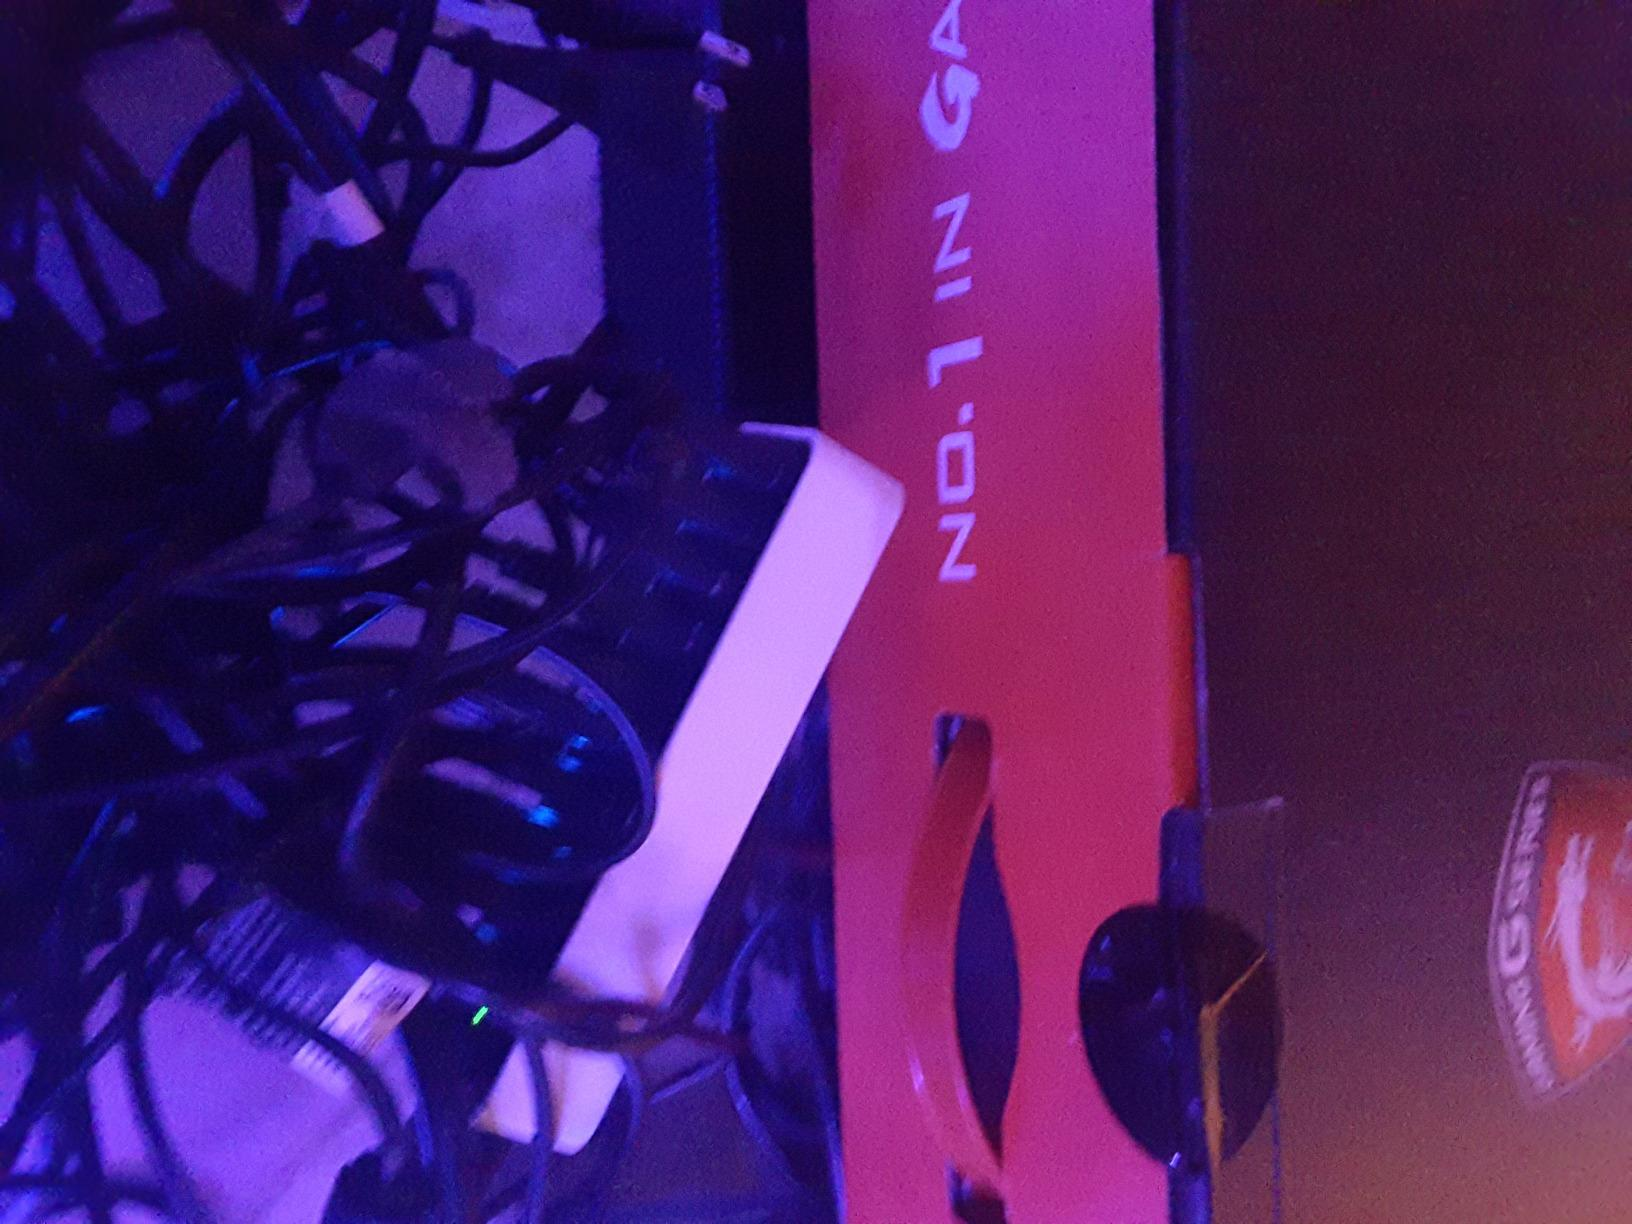
\includegraphics[height=\csfigheight]{Contents/img/case_study/review1/pic_2_1.jpg}} & 1.00 & 0.75 & 0.31 \\
        \bottomrule
        \end{tabular}
    }
    \caption{(Example 1 of 2) Comparison between our model and GBDT on an example from Amazon electronics dataset. The ground truth (GT) scores are annotated ones, while the scores below GBDT and ours are normalized ones.}
    \label{tab:case_study1}
\end{table*}



\begin{table*}[ht!]
    \resizebox{\textwidth}{!}{
        \begin{tabular}{p{0.2\linewidth}|p{0.7\linewidth}}
        \toprule
           Product ID & Introduction \\
         \midrule
            B00H4O1L9Y & Cook food to perfection with the T-fal OptiGrill GC702D53 electric indoor grill. This indoor grill offers versatility and convenience for any grilled meals. Choose from six pre-set programs: Burger, Poultry, Sandwich, Sausage, Red Meat, and Fish. The grills precision grilling technology with sensors measures the thickness of food for auto cooking based on the program selected. When the flashing light turns solid purple, the grill has properly preheatedplace food on the grill, lower the lid, and it takes care of the rest. A cooking-level indicator light changes from yellow to orange to red signifying the cooking progress with audible beeps that alert when food gets to each stage: rare, medium, and well-done. Take food off the grill once its reached your preferred level of doneness. Along with the six pre-set programs, the electric grill provides two additional cooking options: Frozen mode for defrosting and fully cooking frozen food and Manual mode for cooking vegetables or personal recipes. (Note: when preheating for a pre-set program, keep the lid closed or the grill will automatically switch to Manual mode.) The OptiGrill features a powerful 1800-watt heating element, user-friendly controls ergonomically located on the handle, and die-cast aluminum plates with a nonstick coating for effortless food release. The slightly angled cooking plates allow fat to run away from food and into the drip tray for healthier results, and the drip tray and cooking plates are removable and dishwasher-safe for quick cleanup. Housed in brushed stainless steel, the OptiGrill electric indoor grill makes an attractive addition to any counter.  
    
            \subfigure{
\includegraphics[height=\csfigheight]{Contents/img/case_study2/product/pic_4_0.jpg}}
            \subfigure{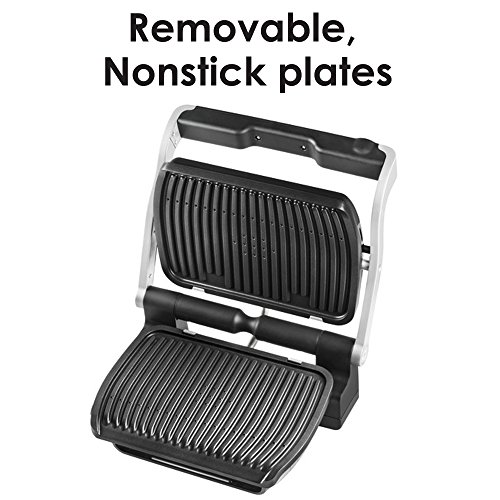
\includegraphics[height=\csfigheight]{Contents/img/case_study2/product/pic_4_1.jpg}}
            \subfigure{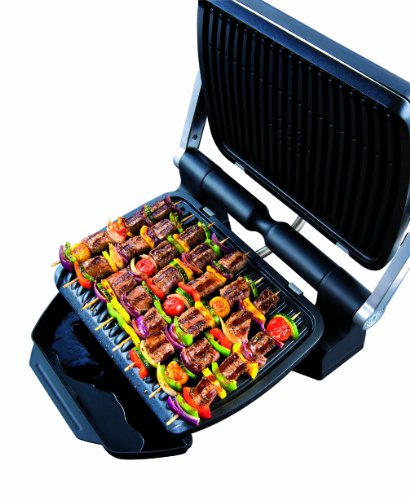
\includegraphics[height=\csfigheight]{Contents/img/case_study2/product/pic_4_2.jpg}}
            \subfigure{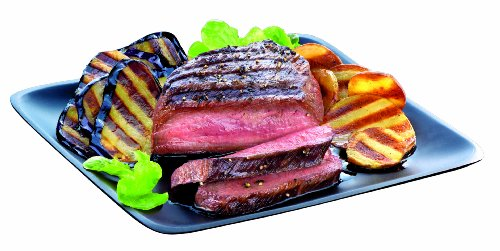
\includegraphics[height=\csfigheight]{Contents/img/case_study2/product/pic_4_3.jpg}} \\
        \bottomrule
        \end{tabular}
    }
    \caption{(Example 2 of 2) Product introduction of an example from Amazon Home dataset.}
    \label{tab:home_product}
\end{table*}

\begin{table*}[ht!]
    \resizebox{\textwidth}{!}{
        \begin{tabular}{p{0.2\linewidth}|p{0.7\linewidth}|p{0.07\linewidth}|p{0.07\linewidth}|p{0.07\linewidth}}
        \toprule
        Review ID & Content & GT & GBDT & Ours \\
        \midrule
        B00H4O1L9Y-111 & 
        I want to preface this by saying that I always prefer food grilled on our big outdoor propane grill.  It's just a superior method of cooking.  That being said, if you don't have an outdoor grill, or even if you do and are sometimes unable to cook with it due to lack of time, running out of propane, inclement weather, laziness...  then this is a FABULOUS option to still get the grilled food you loved SUPER FAST and SUPER EASY!!  We got 5 (yes FIVE) George Foreman grills for our wedding.  I re-gifted 4 of them and kept one and have used it off and on for a long time, but every time I have to clean it afterward I swear I'm never going to use it again because it's such a pain and it never quite gets clean, especially in the area where the hinges are.  That problem is no more....
        
        \subfigure{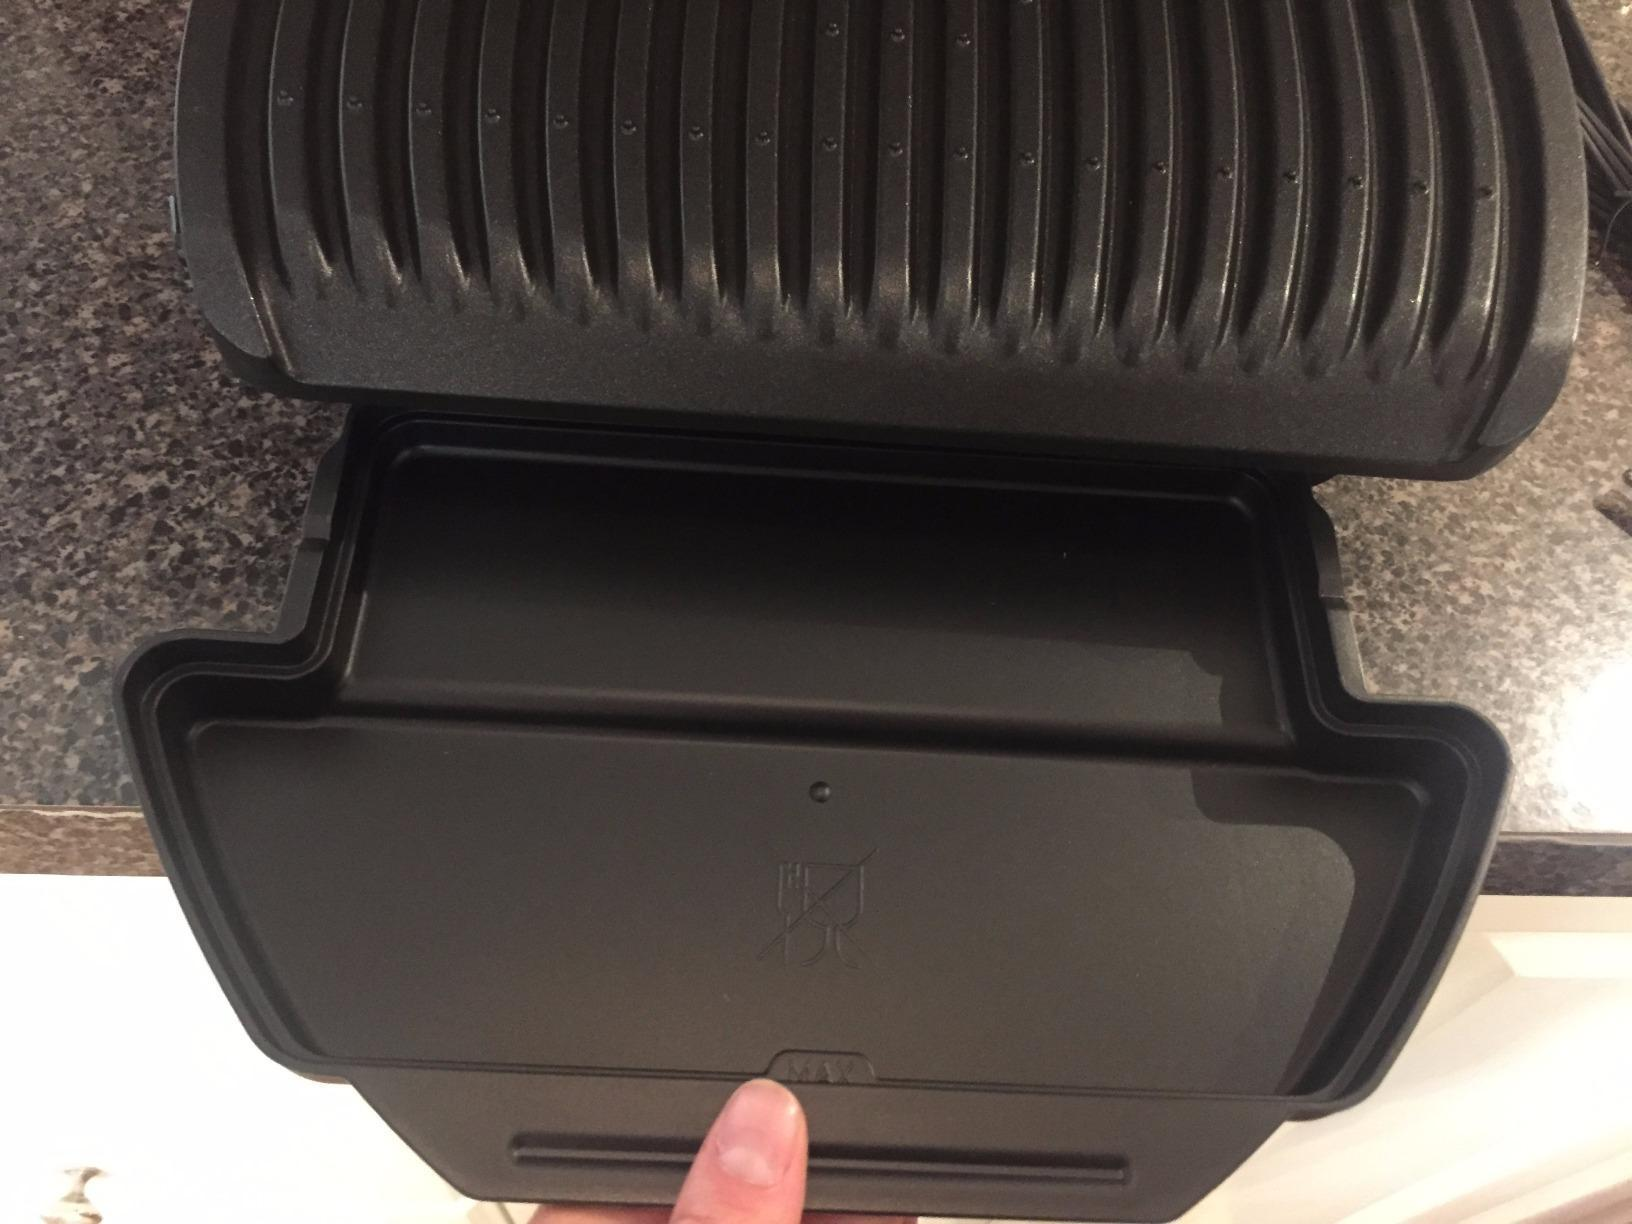
\includegraphics[height=\csfigheight]{Contents/img/case_study2/review4/pic_10_0.jpg}}
        \subfigure{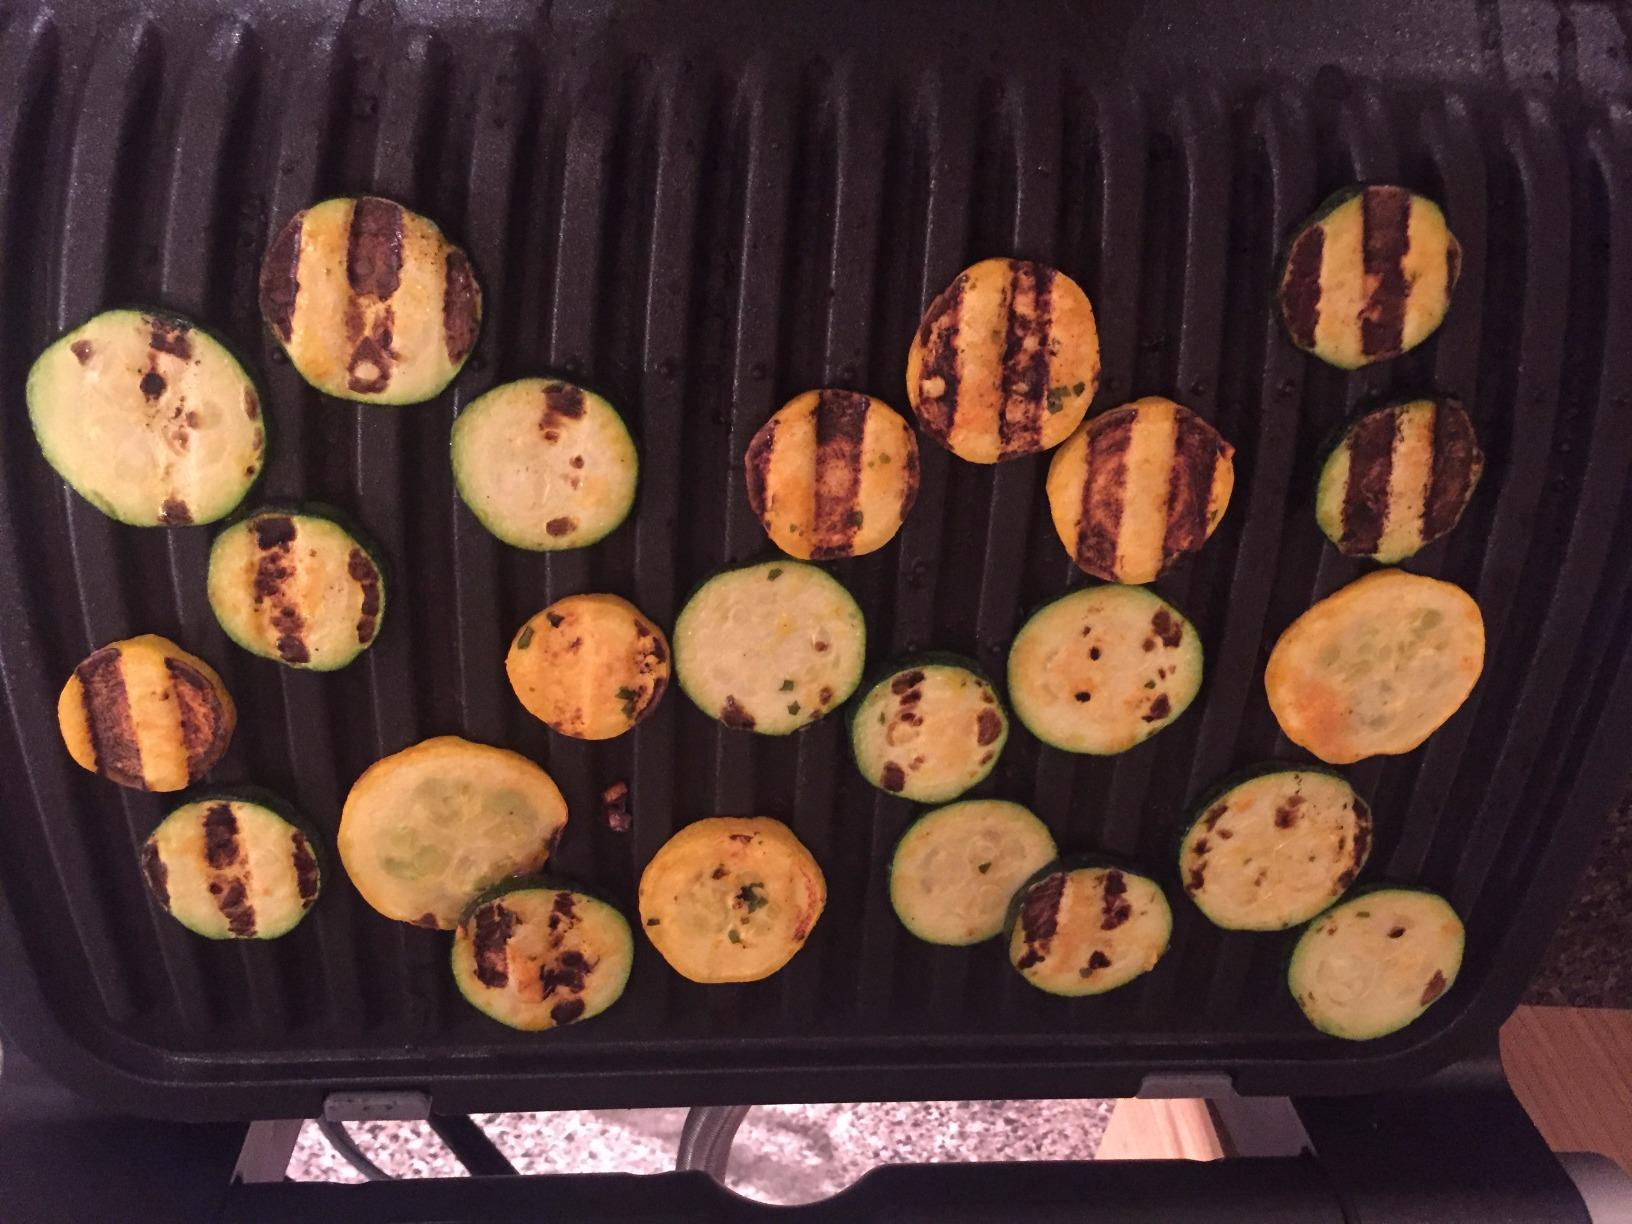
\includegraphics[height=\csfigheight]{Contents/img/case_study2/review4/pic_10_1.jpg}}
        \subfigure{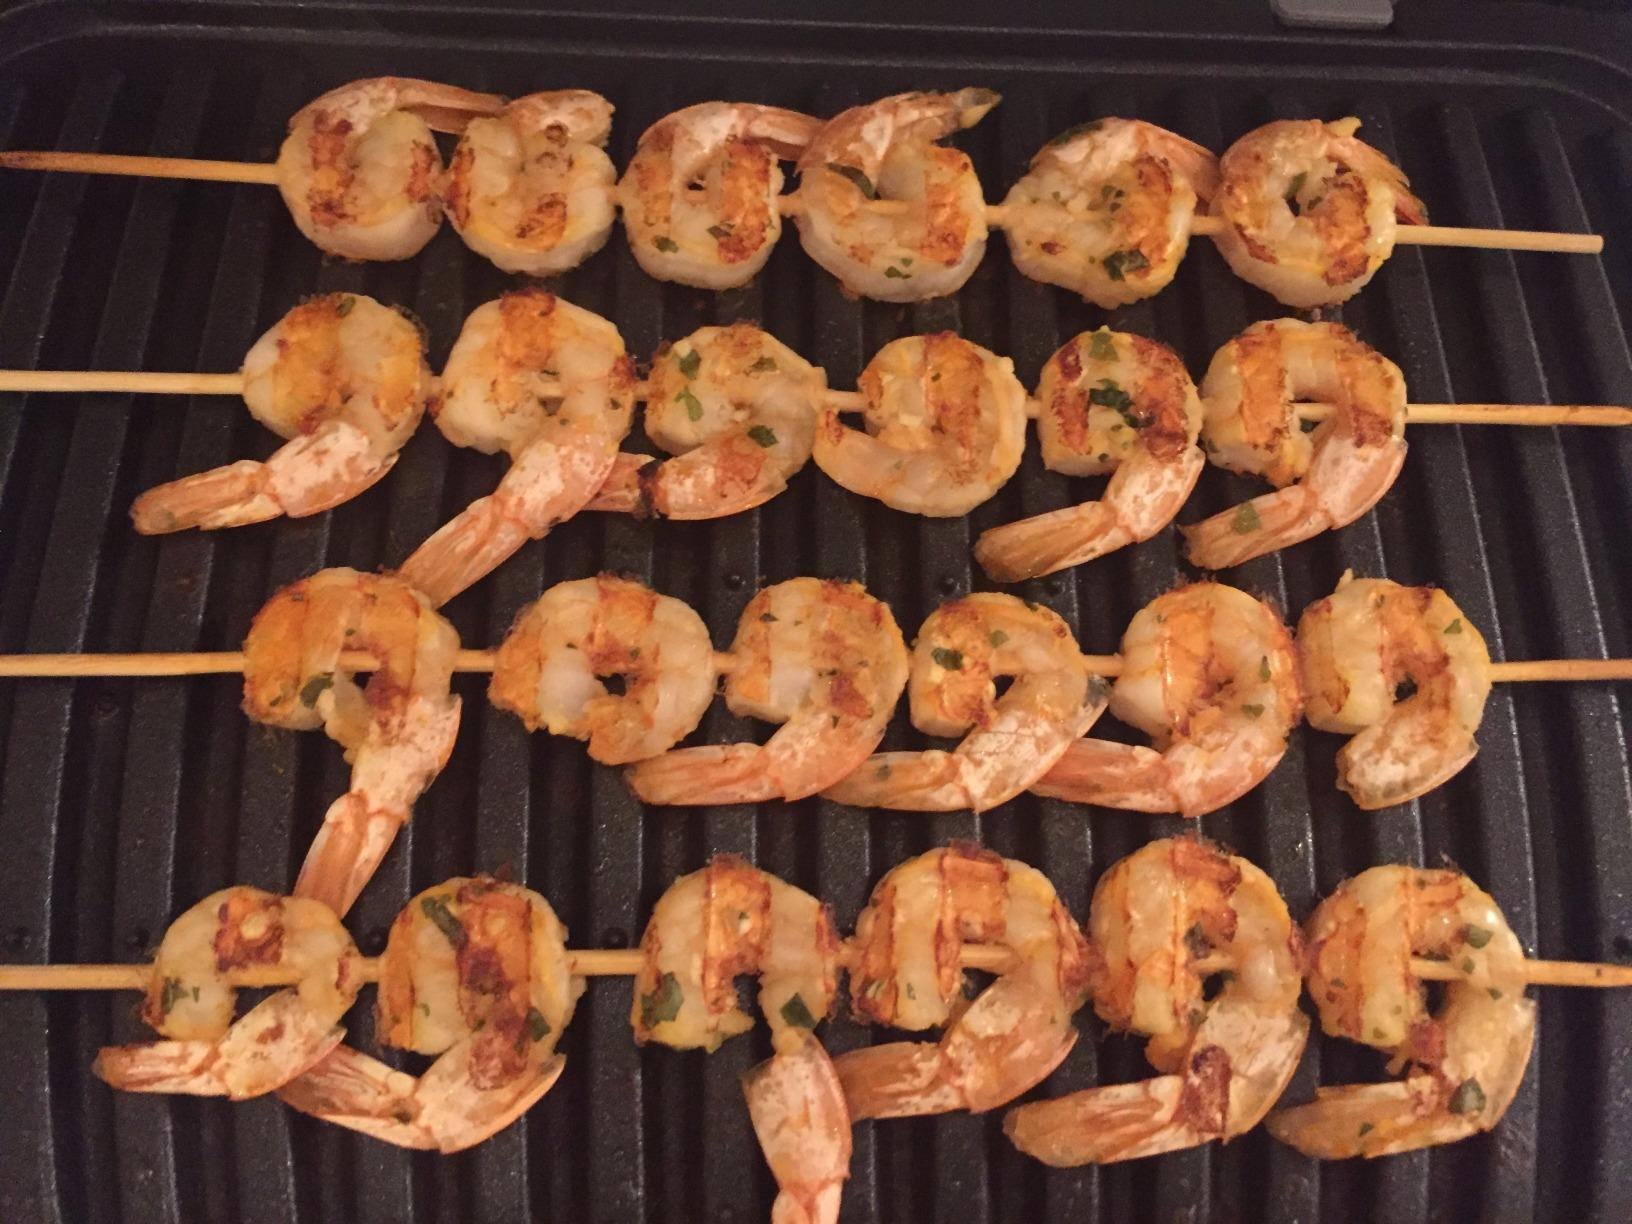
\includegraphics[height=\csfigheight]{Contents/img/case_study2/review4/pic_10_2.jpg}}
        \subfigure{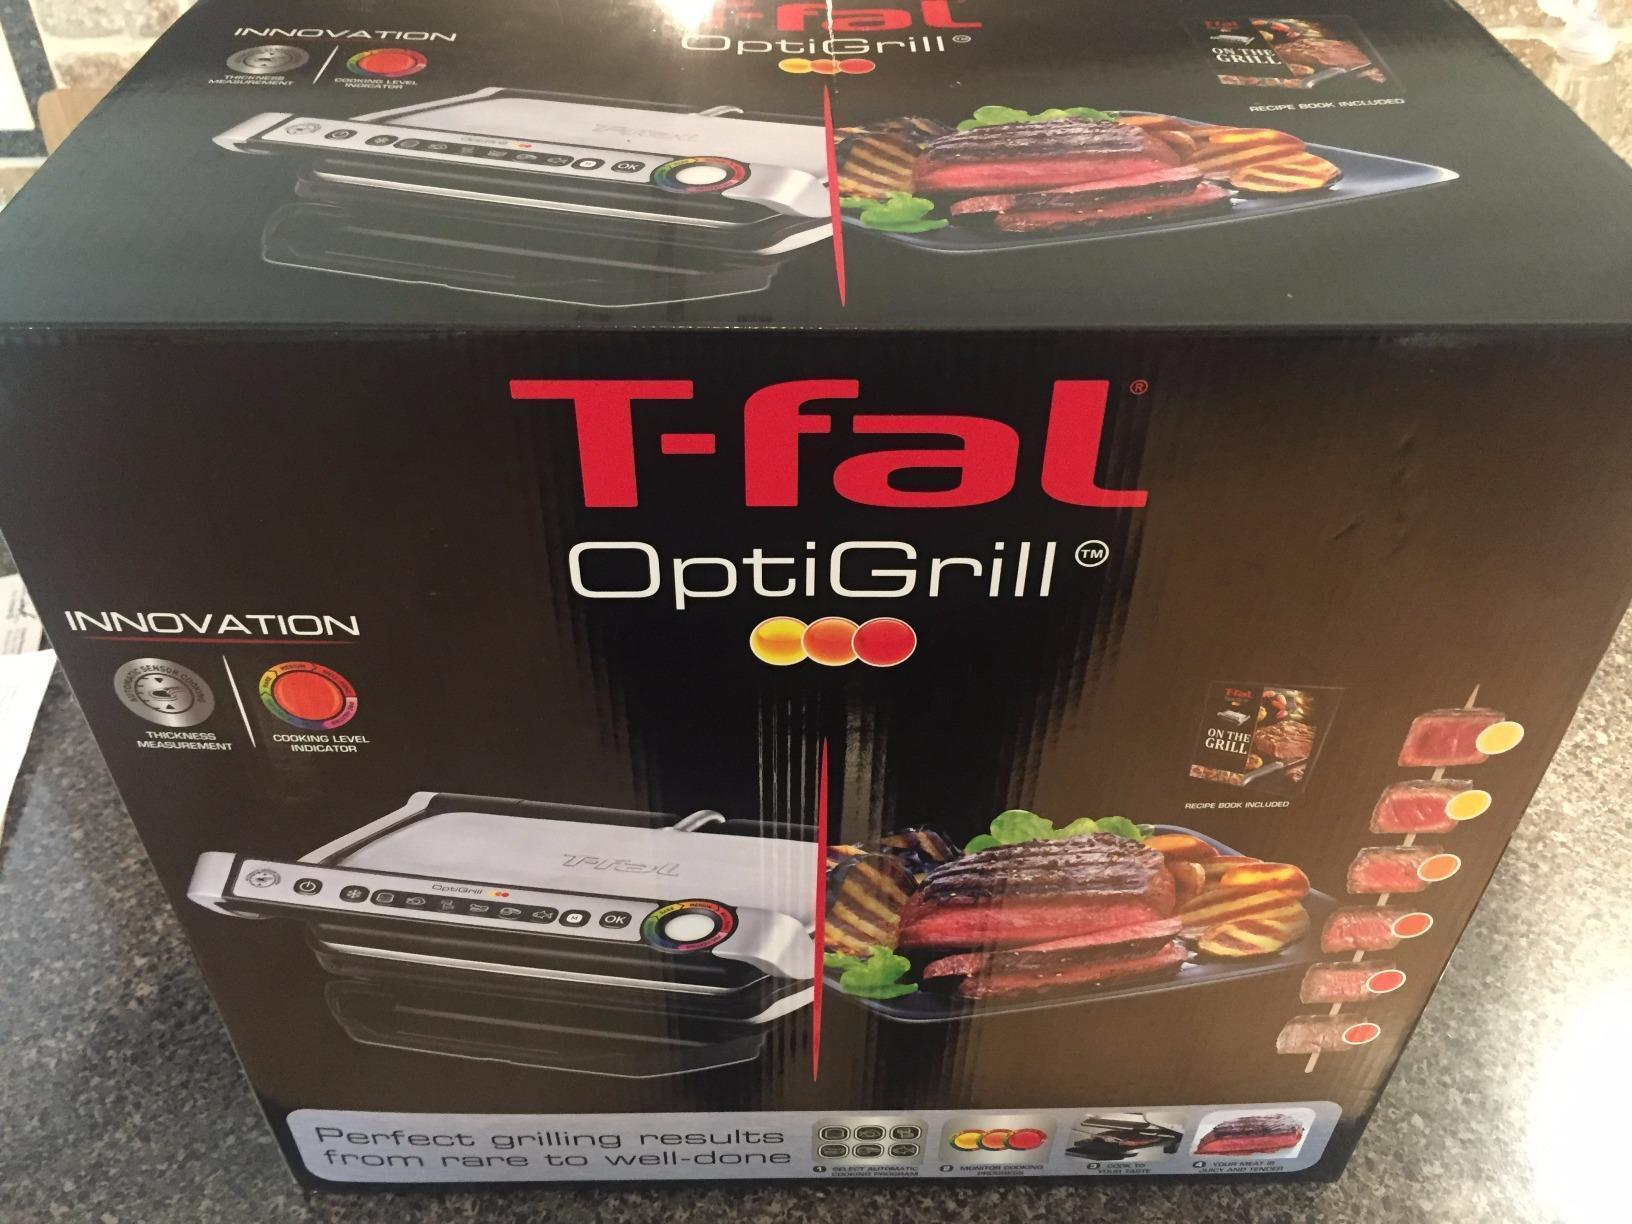
\includegraphics[height=\csfigheight]{Contents/img/case_study2/review4/pic_10_3.jpg}}
        \subfigure{
\includegraphics[height=\csfigheight]{Contents/img/case_study2/review4/pic_10_4.jpg}}
        \subfigure{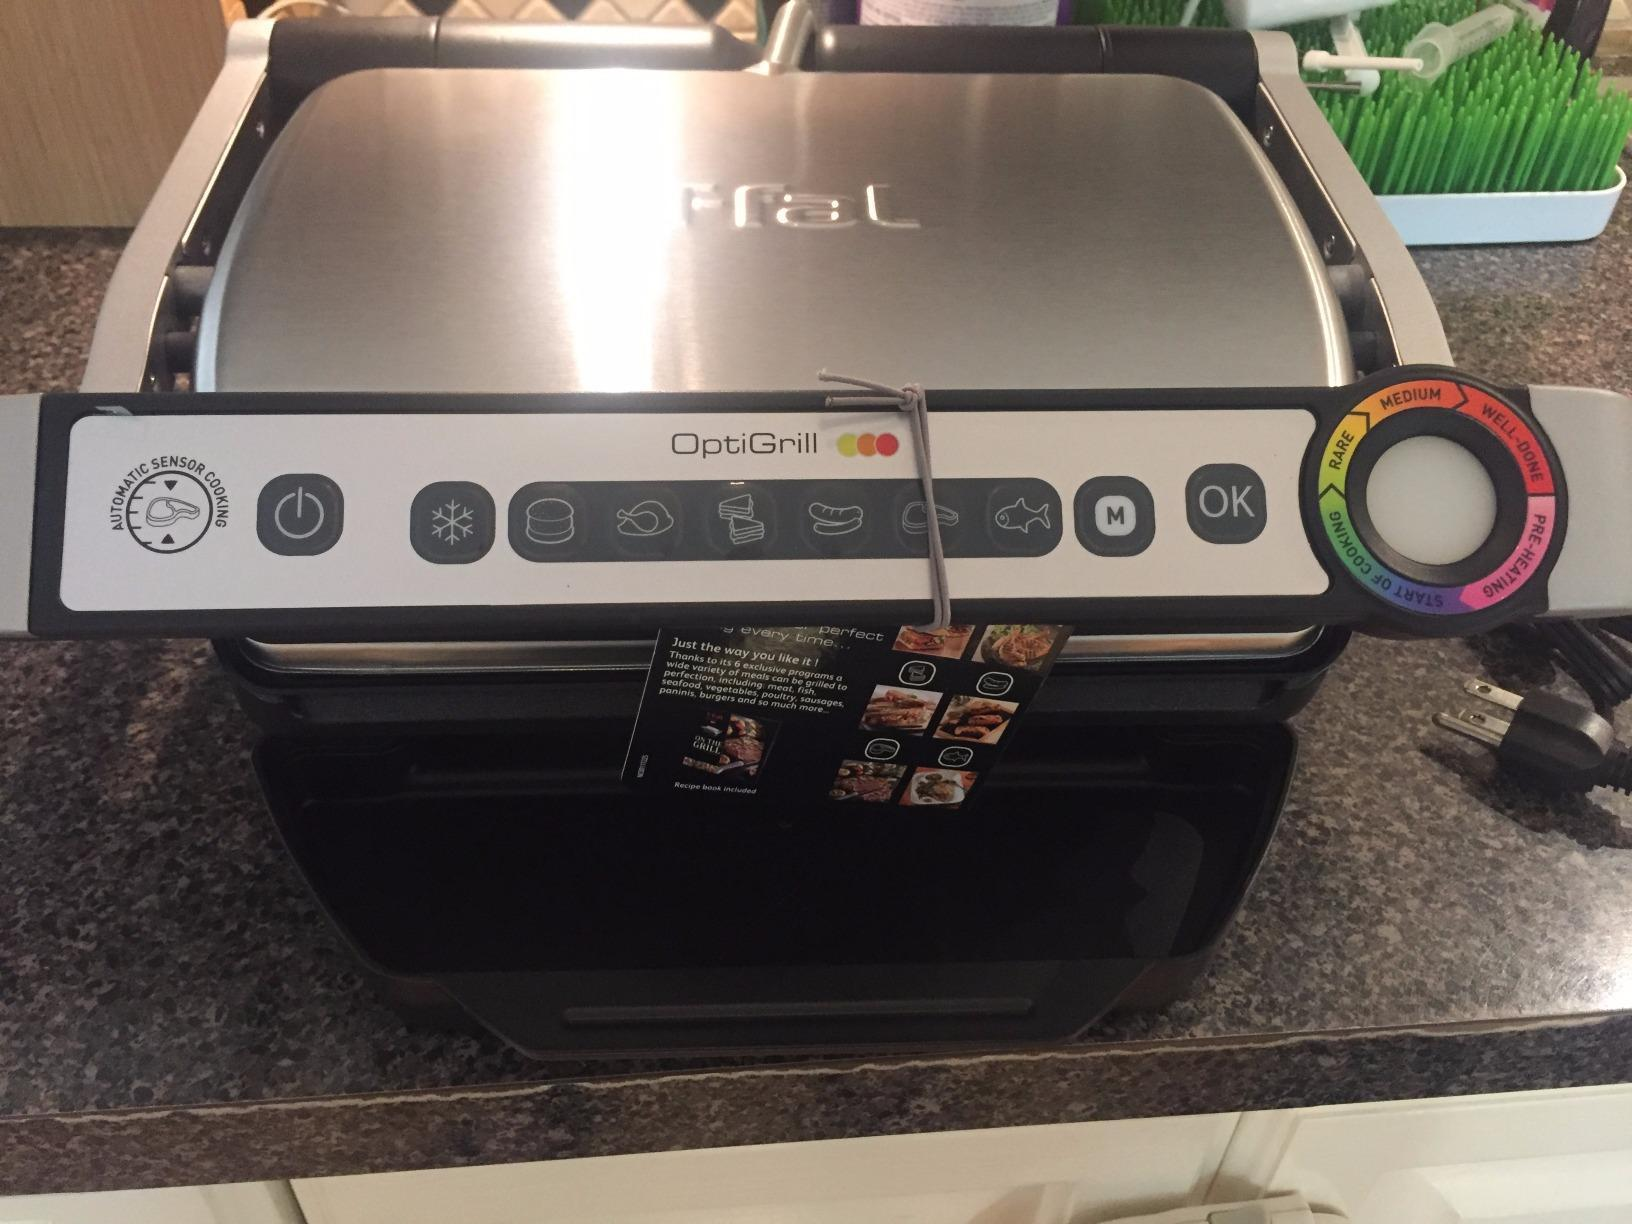
\includegraphics[height=\csfigheight]{Contents/img/case_study2/review4/pic_10_5.jpg}}
        \subfigure{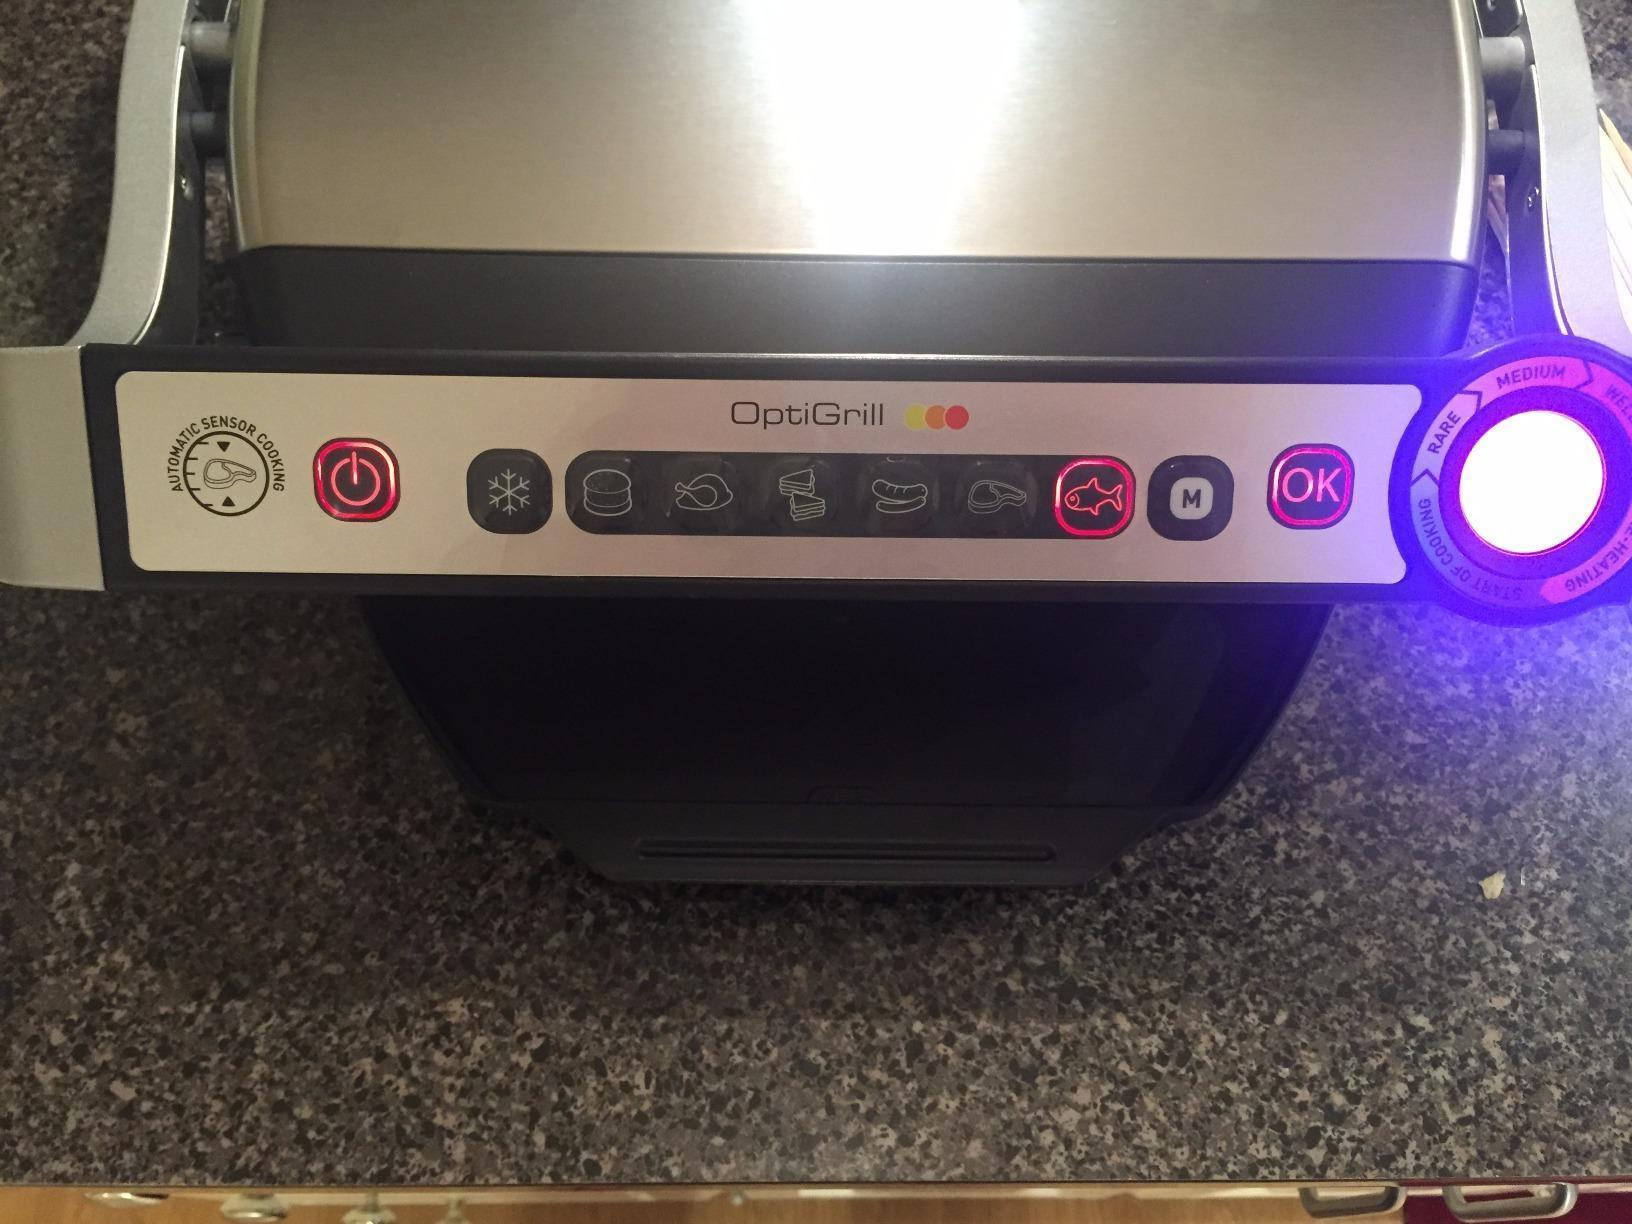
\includegraphics[height=\csfigheight]{Contents/img/case_study2/review4/pic_10_6.jpg}}
        & 4.00 & 0.58 & 0.71 \\
        \midrule
        B00H4O1L9Y-122   &
        My mom got this on her account. I thought she was crazy to spend so much on what looked like a glorified George Foreman grill but I was wrong, this thing is the bomb. Here is what I like about it;-Heats up super quick. I remember my old George Forman grill took a lot longer.-The presets for the type of food you are cooking must be working because nothing turns out overcooked.
        
        The nonstick removable plates. So far, I haven't had any food stick to the plates and I don't use spray or oil. Being able to take them off and wash them in the sink or dishwasher is by far the best part, I used to hate wasting a million paper towels and burning my hands on my old foreman grill and still didn't feel like it was clean. 
        
        Doesn't create a lot of smoke. When I used to use my old foreman grill I was always setting off the smoke alarm, this grill doesn't do that.
        
        \subfigure{
\includegraphics[height=\csfigheight]{Contents/img/case_study2/review3/pic_4_0.jpg}}
        \subfigure{
\includegraphics[height=\csfigheight]{Contents/img/case_study2/review3/pic_4_1.jpg}}
        \subfigure{
\includegraphics[height=\csfigheight]{Contents/img/case_study2/review3/pic_4_2.jpg}}
        \subfigure{
\includegraphics[height=\csfigheight]{Contents/img/case_study2/review3/pic_4_3.jpg}}
        & 3.00 & 0.65 & 0.62 \\
        
        \midrule
        B00H4O1L9Y-148 & I have used this grill 4 times now and everything I've cooked has turned out amazing! I am so impressed with this grill. It is real quick to preheat and has cooked everything perfectly so far from burgers to chicken sausages to kabobs. We haven't tried anything from the cookbook included but we definitely want to. One of the best things is that the plates are detachable and dishwasher safe! Super easy cleanup.
        
        \subfigure{
\includegraphics[height=\csfigheight]{Contents/img/case_study2/review2/pic_2_0.jpg}}
        \subfigure{
\includegraphics[height=\csfigheight]{Contents/img/case_study2/review2/pic_2_1.jpg}} & 2.00 & 0.49 & 0.42 \\
        \midrule
        B00H4O1L9Y-59 & One of the best tools for preparing clean food (if that's what you choose). Cooks in minutes and cleans just as fast. Gives that grill experience within a compact structure. Definitely saves time, I use this thing at least ounce a day, on prep days 3-5 times. If you want to loose wait; it starts in YOUR kitchen by preparing your meals. 
        
        \subfigure{
\includegraphics[height=\csfigheight]{Contents/img/case_study2/review1/pic_4_0.jpg}}
        \subfigure{
\includegraphics[height=\csfigheight]{Contents/img/case_study2/review1/pic_4_1.jpg}}
        \subfigure{
\includegraphics[height=\csfigheight]{Contents/img/case_study2/review1/pic_4_2.jpg}}
        \subfigure{
\includegraphics[height=\csfigheight]{Contents/img/case_study2/review1/pic_4_3.jpg}} & 1.00 & 0.35 & 0.27 \\
        \bottomrule
        \end{tabular}
    }
    \caption{(Example 2 of 2) Comparison between our model and GBDT on the example from Amazon Home dataset. The ground truth (GT) scores are annotated ones, while the scores below GBDT and ours are normalized ones.}
    \label{tab:case_study2}
\end{table*}